%% Problem elaboration
%%=========================================

\chapter{Problem Elaboration}
\label{ch:problem}
Before attempting to solve a problem, it is important to fully understand the problem that is to be solved. In this chapter, we will expand on the problem definition given in the introduction chapter. We examine why the problem may be ambiguous and what that could mean for our system. We will also evaluate different factors and challenges and explain how this may affect our system and how well it functions. Lastly we will look closer at how our problem behaves, and what the relationship between the input and output means. Based on this, we will try to find a conceptual approach to solving the problem.

%%=========================================

\section{Use of Signatures}
As explained in Section \ref{sec:goals_and_research_questions}, our goal is to use a signature to recognize and predict words. Using signatures instead of the entire characters in the word, we have less data to work with. Having less information to work with could mean that our problem is harder to solve. This is not necessarily true in all cases, for example in situations where the rest of the information is misleading or obfuscate in such a way that using it does more harm than good. In such situations it may be better to ignore the additional information altogether. It is difficult to know where these lines goes, as it is difficult to know how certain data will directly or indirectly affect the results ahead of time. In our problem, using exclusively signatures to reorganize words, may open the possibility that the solution sometimes can not be guaranteed, as the input may be ambiguous. While typical character recognition has to deal with misshaped characters, or characters that look suspiciously like other characters, this problem has to deal with input that can be one of many characters, without having the ability to differentiate between them. This is explained further in Section \ref{sec:ambiguous_input}.

%%=========================================

\section{Tuning Input Data}
\label{sec:tuning_input_data}
With the use of signatures, we can alter how we capture the data from the original image in a number of ways. The alterations can be done by configuring text sizes, signature positions, or signature heights in different ways. Altering the signature capturing configurations would result in completely new sequences for words.

\begin{figure}[ht]
    \centering
    
\includegraphics[width=0.7\textwidth]{fig/chapter2/signature_multiple.png}
    \caption{The word ``CAT" with two signatures at different heights}
    \label{fig:thesis-signature-comparison}
\end{figure}

Let us consider the word ``CAT" in upper-cased letters, written in Arial with a font height of 50 pixels, as illustrated in Figure \ref{fig:thesis-signature-comparison}. In this figure, we have highlighted two signatures, both with the height of one pixel. The first signature is 16 pixels from the bottom, while the other is 45 pixels from the bottom. As we can see from the illustration, the signatures we capture from the text varies significantly depending on where we chose to place it. For example, the top signature defines a ``T" as 38 black pixels, while the bottom defines it as seven black pixels.

Figure \ref{fig:thesis-signature-comparison} also illustrates how our system needs to differentiate between letter spacing and characters that consists of white space. In the bottom signature, the letter ``C" is defined as a sequence of eight black, 27 white, and seven more black pixels. However, the sequence of seven black, seven white and 35 more black pixels is just the final stroke of the letter ``C" as well as the letter ``A" including the space between the two letters. This sequence should not be classified as a letter, as it contains fragments of two separate ones. These examples illustrates how small adjustments in the capturing of signatures makes the sequences vary.

%%=========================================

\section{Use of Fonts}
\label{sec:use_of_fonts}

\begin{figure}[h]
    \centering
    
\includegraphics[width=1.0\textwidth]{fig/chapter2/typeface_comparison.png}
    \caption{The word ``CAT" in Arial and Times New Roman with highlighted serifs}
    \label{fig:typeface-comparison}
\end{figure}

In addition to alterations of the input data, as explained in section \ref{sec:tuning_input_data}, choice of font may also play a role in the ambiguity of the problem. In Figure \ref{fig:thesis-signature-comparison} we have used the monolined sans-serif font Arial. Monoline means that the strokes in the typeface have the same widths throughout. Sans-serif means that the font does not have serifs; a crossing feature at the end of the principal character strokes \citep{felici2011complete}. In Figure \ref{fig:typeface-comparison} we have again written the word ``CAT" first in Arial, and then in Times New Roman. Times New Roman is a font with serifs which is not monolined. The serifs are highlighted in red. The visual difference between the two words illustrates how the choice of font affects the captured sequences.

\begin{figure}[ht]
    \centering
    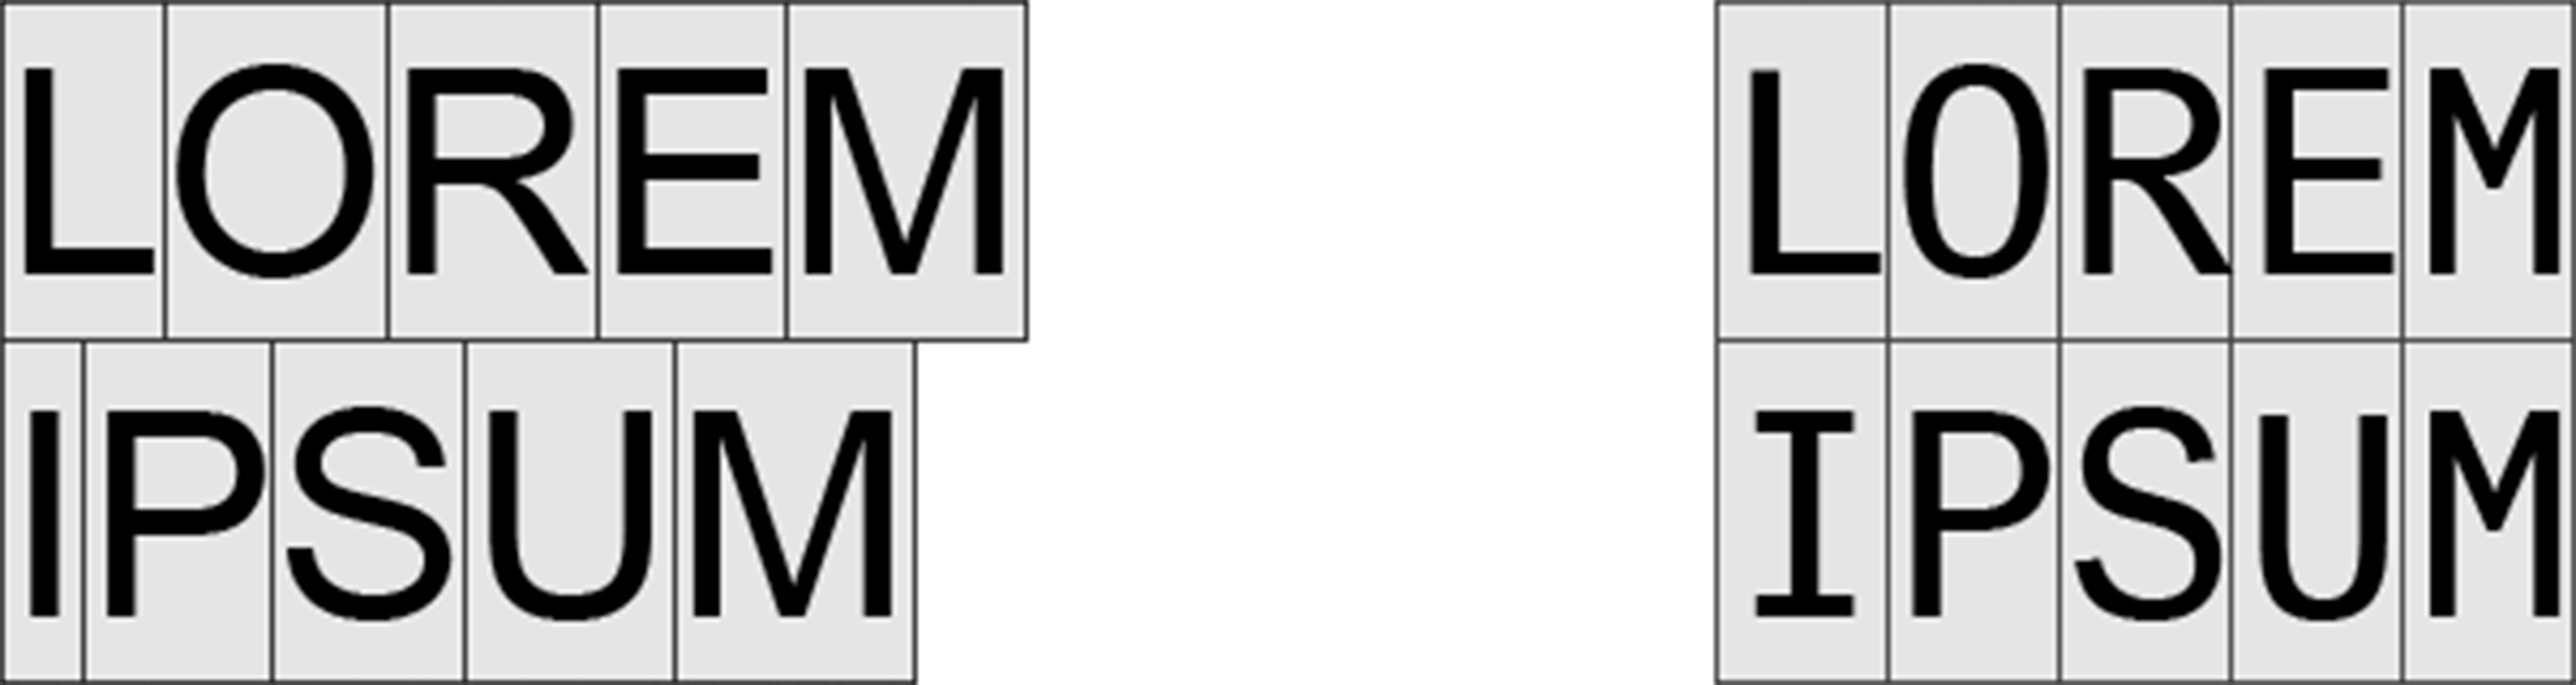
\includegraphics[width=1.0\textwidth]{fig/chapter2/regular_mono_comparison.png}
    \caption{Text with a variable-width font on the left, and monospace on the right}
    \label{fig:regular-mono-comparison}
\end{figure}

In addition to the variances already mentioned, there are there also differences in how fonts are spaced. A monospaced font, also called fixed-width font, uses the same width for all characters. This is in contrast to variable-width fonts, where each character may have different widths \citep{felici2011complete}. Illustrated in Figure \ref{fig:regular-mono-comparison}, the text on the left is written in regular Arial which has variable width characters, while the text on the right is written in a Arial variant with monospacing. In the text on the right each letter in the two words match each other in widths, while the varying widths of the glyphs in the text to the left causes the letters to be shifted. With a monospaced font, each glyph is placed inside a maximum width constraint. The glyph does not need to take up the entire width, but guarantees that there are no strokes outside the constraint. In our problem, we do not define where a character ``starts" or ``stops", so we do not know the location of these constraints. This means that there will be variance in the distance from one glyph to another depending on which characters they represent. However, the variance will be more significant in a font that has variance-width. 

%%=========================================

\section{Other Factors}
\label{sec:other_factors}
There are even more factors that play a role in how the fonts look, which will also affect the characteristics of the captured sequences. Kerning is one such factor. Kerning is the process of adjusting the spacing between two characters to compensate for their relative shapes. This is done to increase the readability and create a more visually pleasing result \citep{felici2011complete}. An illustrative example of kerning can be seen in Figure \ref{fig:kerning-comparison}, where the letters on the left side has applied kerning, bringing the two letters closer. The letters on the right side has no kerning. On the left side, the letters more naturally fit against each other, while the letters on the right side have a conspicuous spacing between them. As for our problem, kerning may make it more difficult to separate the characters from each other. Because kerning eliminates long sequences of spacing, by shifting characters closer to each other, it eliminates ``hints" that could otherwise be used to identify where one letter ends and another begins.

\begin{figure}[ht]
    \centering
    
\includegraphics[width=1.0\textwidth]{fig/chapter2/kerning.png}
    \caption{Kerning adjusted text on the left, no kerning on the right}
    \label{fig:kerning-comparison}
\end{figure}

\newpage
There are even more techniques in typography that are applied to text to get the more readable and visually pleasing arrangements of characters. As these alter how the text looks, it also alter our input data. Some of these are \citep{felici2011complete}:

\begin{itemize}
    \item Typographic alignments, such as justified text or ragged right.
    \item Font weights, which defines the degree of boldness and widths of strokes.
    \item Slanted forms such as italic.
    \item Location of the baseline, which defines the line that most of the characters appear to be sitting on.
    \item Anti-aliasing or font smoothing, which is a technique to smoothing the appearance of characters on a computer screen by adding gray pixels around their edges.
\end{itemize}

%%=========================================

\section{Ambiguous Input}
\label{sec:ambiguous_input}
There is a chance our input data may end up being ambiguous, or at least ends up being so complicated it becomes be very difficult to decode and learn properly. A character signature can consist of a single sequence of black pixels, or a series of alternating black and white pixels. Because our system does not know exactly what a character looks like, there is no way for it to know what sequences are ``rests" of characters, spacing, or valid characters. It may also happen that a character consisting of a single sequence of black pixels is also a subset of another character. 

Consider the lower signature in Figure \ref{fig:thesis-signature-comparison}. Because Arial is monolinear, we know that the strokes on the ``C" and the ``T" have equal width. The ``T" could be represented as a series of some white pixels, three black pixels, and optionally more white pixels. We can not know for sure just how many white pixels is before and after the three black pixels, because this may vary depending on what character is before and after the ``T", if any. Now, if our system learns this definition, it will incorrectly label various other characters, such as parts of the ``C" as a potential ``T". This means that our system has to learn the recognize a huge variety of sequences and correctly map them to an output character.

\begin{table}[H]
    \centering
    \begin{tabular}{|l|l|l|}
        \hline 
        \textbf{Character(s)} & \textbf{Signature}                                    & \textbf{Sequence}            \\ \hline
        A                     & \([0, 0, 0, 1, 1, 1, 1, 1, 1, 1, 0, 0, 0]\)             & \(3B, 7W, 3B\)                 \\ \hline
        B                     & \([0, 0, 0, 1, 1, 1, 1, 1, 1, 1, 0, 0, 0, 0, 0]\)       & \(3B, 7W, 5B\)                 \\ \hline
        C, I, J, L, T and Y   & \([0, 0, 0]\)                                           & \(3B\)                         \\ \hline
        D                     & \([0, 0, 0, 1, 1, 1, 1, 1, 1, 1, 1, 1, 1, 0, 0, 0]\)    & \(3B, 10W, 3B\)                \\ \hline
        E and F               & \([0, 0, 0, 0, 0, 0, 0, 0, 0, 0, 0, 0, 0, 0]\)          & \(14B\)                        \\ \hline
        G                     & \([0, 0, 0, 1, 1, 1, 1, 1, 1, 0, 0, 0, 0, 0, 0, 0, 0]\) & \(3B, 6W, 7B\)                 \\ \hline
        H and U               & \([0, 0, 0, 1, 1, 1, 1, 1, 1, 1, 1, 1, 0, 0, 0]\)       & \(3B, 9W, 3B\)                 \\ \hline
        K                     & \([0, 0, 0, 0, 0, 1, 0, 0, 0, 0]\)                      & \(5B, 1W, 4B\)                 \\ \hline
        M                     & \([0, 0, 0, 1, 1, 1, 1, 0, 1, 1, 1, 1, 0, 0, 0]\)       & \(3B, 4W, 1B, 4W, 3B\)         \\ \hline
        N                     & \([0, 0, 0, 1, 1, 1, 1, 0, 0, 0, 1, 1, 0, 0, 0]\)       & \(3B, 4W, 3B, 2W, 3B\)         \\ \hline
        O and Q               & \([0, 0, 0, 1, 1, 1, 1, 1, 1, 1, 1, 1, 1, 1, 0, 0, 0]\) & \(3B, 11W, 3B\)                \\ \hline
        P                     & \([0, 0, 0, 0, 0, 0, 0, 0, 0, 0, 0, 0, 0]\)             & \(13B\)                        \\ \hline
        R                     & \([0, 0, 0, 0, 0, 0, 0, 0, 0, 0]\)                      & \(10B\)                        \\ \hline
        S and X               & \([0, 0, 0, 0, 0, 0, 0]\)                               & \(7B\)                         \\ \hline
        V                     & \([0, 0, 0, 0, 1, 1, 1, 1, 0, 0, 0]\)                   & \(4B, 4W, 3B\)                 \\ \hline
        W                     & \([0, 0, 0, 1, 1, 1, 0, 0, 1, 0, 0, 0, 1, 1, 0, 0, 0]\) & \(3B, 3W, 2B, 1W, 3B, 2W, 3B\) \\ \hline
        Z                     & \([0, 0, 0, 0]\)                                        & \(4B\)                         \\ \hline
    \end{tabular}
    \caption{Example of signatures and sequences for the uppercase letters in the English alphabet}
    \label{table:signature_sequence_example}
\end{table}

Table \ref{table:signature_sequence_example} holds the actual signatures and sequences for monospaced Arial given the settings specified in section \ref{sec:goals_and_research_questions}. This table illustrates how the input looks and what our system has to decode and learn. As mentioned before, this problem may be very difficult, if not impossible, to learn fully. We can see examples of why it may be difficult in the sequences for the letters C, I, J, L, T, and Y. These six letters all share the same sequence. With an identical sequence, the only way we can differentiate them is to consider the white pixels before and after the three black pixels.  In addition, many of the other character sequences besides the ones for C, I, J, L, T, and Y contains three black pixels after each other. In total, the subsequence of three black pixels is found in eleven of the seventeen unique character sequences. Some of them, like W and N, also contains three subsequent black pixels multiple times in their sequences. 

We also have to remember that the sequences in this table are just the sequences that corresponds to valid characters. Once we have multiple characters after each other, with the natural spacing between them, many new sequences also have to be considered. 

This all boils down to the fact that the complete sequences for words may have many repeated subsequences, where some of them are individual letters, while other are parts of multiple ones. This substantiates that correctly recognizing letters in words using signatures is a difficult problem that requires a system that is able to learn beyond simply reorganizing parts of the sequences.

%%=========================================

\section{Evaluating Problem Input and Output}
\label{sec:evaluating_problem_input_and_output}
In our particular problem we have an input that is a matrix or a vector of binary data. The binary input denotes the color of a particular pixel at the given location in our ``signature". The output, or the correct labels, will correspond to the correct letter in the word. For convenience, the letters will be given a unique integer value. For example, if the words are written in upper cased letters of the English language, we could want our output to be in the range 1 to 26, denoting A to Z.

\begin{figure}[h]
    \begin{equation}
        \label{eq:input_output_example}
        \begin{aligned}
           \vec{\text{inputRaw}}               &= \lbrack 4W, 3B, 7W, 3B, 8W, 3B, 18W, 3B, 23W, 3B, 13W, 14B, 6W, 3B, 10W, 3B \rbrack \\
           \vec{\text{inputEncoded}}           &= \lbrack 4, -3, 7, -3, 8, -3, 18, -3, 23, -3, 13, -14, 6, -3, 10, -3 \rbrack \\
           \vec{\text{outputEncoded}}          &= \lbrack 1, 12, 12, 9, 5, 4 \rbrack \\
           \text{output}                       &= \text{ALLIED}
        \end{aligned}
    \end{equation}
    \captionsetup{labelformat=empty}
    \caption{Input and output example}
\end{figure}

\ref{eq:input_output_example} contains an example with inputs and outputs for the word ``ALLIED". Note that in this example, we have also encoded the input to whole integers. We did this by negating the lengths of sequences of black pixels. This means that four black pixels are encoded as $-4$. Similarity, sequences of white pixels were not altered, so 18 white pixels would be encoded as $18$. This encoding was done to have easier data to work with. 

\subsection{Input Format}
Our input has the feature that they form a sequence. Both the values in the sequence, and the ordering of the sequence is crucial for prediction. This is fundamentally different from other problems such as traditional image recognition, where the exact location of a pattern is not important.

Because the input forms a sequence, it is important that the entire sequence is read, and that we do not cut the sequence off at the end, removing important information that we need. Truncating or ignoring a values in the input sequence would result in mislearning. Instead of our model correctly identify subsequences, the model would attempt to find patters in the data that is not there. This would cripple the model and the overall accuracy may suffer due to contradicting sequences. Keeping the input data unaltered and complete is therefore essential.

\begin{figure}[h]
    \begin{equation}
        \label{eq:input_stop_words}
        \begin{aligned}
           \vec{\text{inputEncoded}}                &= \lbrack -3, 23, \pi, -3, 13, \pi, -14, \pi \rbrack \\
           \vec{\text{outputEncoded}}               &= \lbrack 12, 9, 5 \rbrack \\
           \text{output}                            &= \text{LIE}
        \end{aligned}
    \end{equation}
    \captionsetup{labelformat=empty}
    \caption{Input with stop words}
\end{figure}

We also lack the concept of ``stop words" in our problem. Example \ref{eq:input_stop_words} illustrates an input with stop words, denoted as $\pi$. Stop words may make the problem easier to solve, as as we would know within which boundaries each character resides. In example \ref{eq:input_stop_words}, we have placed the stop word right before the beginning of a new character, instead of just the barriers of the character itself. This could potentially reduce ambiguity as we would now know for a fact that the letter I, if followed by an E, would always be the subsequence \([-3, 13]\). Instead of relying on stop words, we want our model to find a pattern in the sequence data that makes sense based on the corresponding output. This pattern, if correctly predicted, would not need explicit stop words, as the model should be able to find them implicitly.

\subsection{Output Format}
As with the input, our output also form a sequence. Both the values in the sequence, and the ordering of the sequence, is important. The words `HELLO` and `HLLOE` contains the same letters, but have a different meanings. Understanding that both the individual values in the output sequence, as well as the placement of each of them, is important for understanding how our problem is different from many others.

%%=========================================

\section{Translation}
We have now considered the input and output separately. Considering them ``together" we can see the relationship between the two. Sequences and subsequences in the output results in an output sequence or single output value. We can look at this process as a type of translation. We ``translate" the input sequences of language \(\alpha\) into an output sequence of language \(\beta\). It is irrelevant that the actual input and output are not defined language with linguistic properties. As long as there is a relationship between the two ``languages", the task may be considered as a type of translation between the two. Figure \ref{fig:number_translation} illustrates the translation between our two languages, reusing the data from Example \ref{eq:input_stop_words}. The values in the translated language is the same as the encoded output in \ref{eq:input_stop_words}, that is, the index value for each letter in the English language, where ``A" is one, ``B" is two and so on.

\begin{figure}[h]
    \centering
    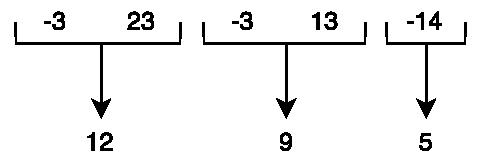
\includegraphics[width=0.7\textwidth]{fig/background_theory/number_translation.pdf}
    \caption{Illustrative translation between our two languages}
    \label{fig:number_translation}
\end{figure}

\subsection{Dissimilarities to Typical Translation Problems}
While our problem may be very similar to that of translation, it also differs in several ways. Common for almost all of these differences is that our languages are very simple. This means that we can simplify, or completely ignore, tasks that are otherwise important in more complex translation problems. For example, the task of ``part-of-speech tagging" is to determine the part of speech for each word in a sentences. This means to determine if a word is a noun, verb, adjective, and so on. This is a complex task, and a task that is important to get right. In our constructed ``languages", we have no concept of such speech groups. Our ``words" has one, and only one, meaning, regardless of context. In addition, translating a sentence from one spoken language to another spoken language does not give any guarantees in the ordering of the words. Words that can be directly translated between the languages does not necessarily have the same arrangement in both of them. This is due to how languages structure their sentences. For our language, we know that the ordering will always be the same. Although the length of the language will vary between input and output, we know that a certain value in the input will not affect an output that it does not map to. Reusing the input and output from example \ref{eq:input_stop_words}, we know that the input subsequence \([-3, 23]\) maps to the output \(12\), and it can not affect the values of \(9\) or \(5\).

These observations makes it clear that although our problem is related to translation, it also differs from more traditional problems. These differences will make it interesting to see how well a translation based model can handle our problem.